The NW algorithm works by populating a matrix from the north-western corner towards the south-eastern corner. Which in practicality means that, to determine the value of any number in the matrix, the western, northern and north-western value needs to be computed first.

So the work needs to be partitioned in a non-trivial way to maximize the processor power used in a multiprocessor environment.

A tiling approach was here explored\cite{TODO}, with the thought being of dividing the computation matrix into a number of tiles, the power of these tiles is that we can decide their size, and thus optimize it to the given cahches size of the multiprocesssor environment we are working in.

Another power of these tiles is that, as individual values, a tile can be calculated if the western, southern and south-western tile has been computed This leads us to the order in which these tiles will be computed, which is described in Figure \ref{fig2}. Every diagonal strip of tiles will be able to be computed concurrently, which means that for a large enough amount of tiles, the amount of processors that can be active will be incremented by one for every strip, until the strips narrow down in size.
\begin{figure}[H]
  \center
  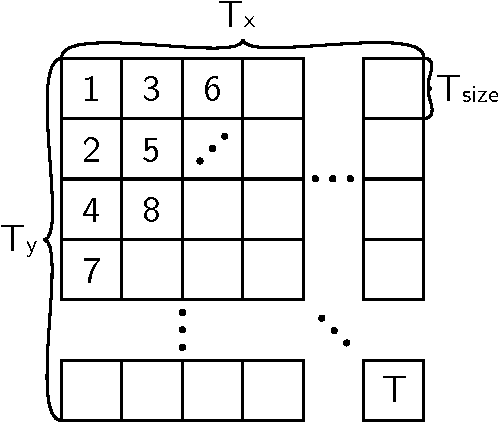
\includegraphics[width=0.4\textwidth]{fig/fig2.pdf}
  \caption{The ordering the tiles are computed in.}
  \label{fig2}
\end{figure}
Every tile will be responsible for computing three things, its southern edge, eastern edge and the south-eastern corner, which it will be able to feed to its respective neighbouring tiles. This input-output relationship is shown in Figure \ref{fig1}, this figure also shows the input corner, which is always 0, and it output corner, which is the final output of the algorithm.
\begin{figure}[H]
  \center
  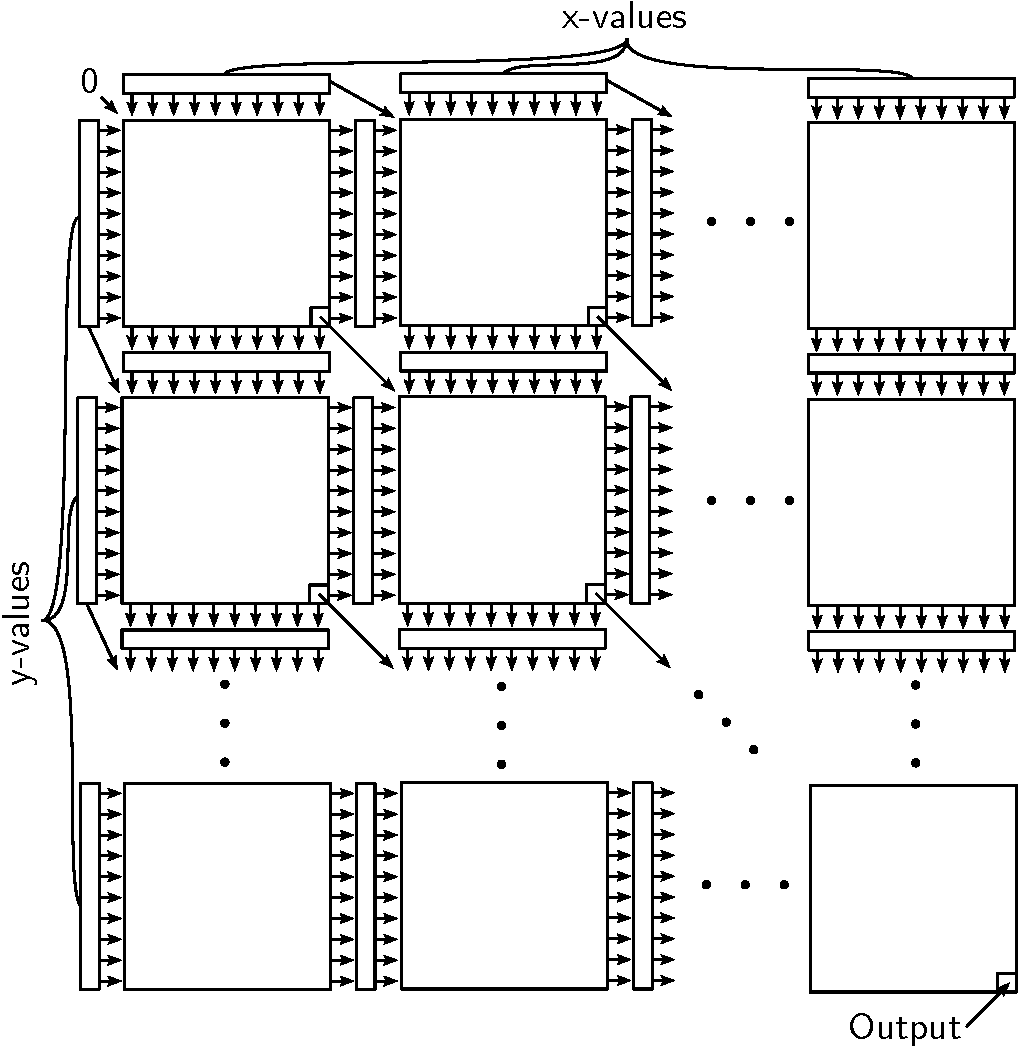
\includegraphics[width=0.7\textwidth]{fig/fig1.pdf}
  \caption{The input and output of the tiling structure. Each tile here will populate their western and northern edges using their input arrays and input corner, their output will be their eastern and southern edges and their south-eastern corner.}
  \label{fig1}
\end{figure}
The way this is structured ensures there is only a memory usage of $P\cdot T_{size}^2$, where $P$ is the amount of processors, and $T_{size}$ is the length of a tiles size, which is important in dealing with large inputs, as the entire solution matrix is never in memory at the same time. The also implies that the solution to reach the best alignment, is lost, only the final score is reported.
